\documentclass[a0, portrait]{a0poster}
\usepackage[english]{babel}
\usepackage[utf8]{inputenc}
\usepackage[T1]{fontenc}
\usepackage{siunitx, multicol, xcolor, float, enumerate, cite, url}
\usepackage{helvet}
\usepackage[left=50pt, right=50pt, top=50pt, bottom=50pt]{geometry}
\usepackage[framemethod=TikZ]{mdframed}
\usepackage[font=small,labelfont=bf]{caption}

\input{/home/istvan/insar/latex_aux.tex}

\columnsep=80pt
\columnseprule=2.5pt

\graphicspath{{/home/istvan/work/insar/images/}}
\DeclareGraphicsExtensions{.png,.jpg,.jpeg}

\global\mdfdefinestyle{title}{%
    linecolor=black, linewidth=3pt,
    innerleftmargin=10pt, innerrightmargin=10pt,
    innertopmargin=25pt, innerbottommargin=25pt,
    backgroundcolor=black!10!white
}

\renewcommand{\familydefault}{\sfdefault} % helvetica font

\begin{document}

%-----------------------------------------------------------------------
% TITLE
%-----------------------------------------------------------------------

\bfseries

\begin{mdframed}[style=title]
    \hspace{25pt}
    \begin{minipage}[c]{0.2\textwidth}
        
\includegraphics[width=12.5cm]{ggi_logo.png}
    \end{minipage}
    \hspace{-50pt}
    \begin{minipage}[c]{0.6\textwidth}
      \Large {\color{blue!30!black} ESTIMATION OF NEARLY VERTICAL AND EAST-WEST SURFACE DEFORMATION VELOCITY COMPONENTS USING ARCHIVE ENVISAT SAR IMAGES PROCESSED WITH PERSISTENT SCATTERERS INTERFEROMETRY}\\[25pt] % Title
    István Bozsó, Eszter Szűcs, László Bányai, Viktor Wesztergom \\[10pt]% Author(s)
     \large \normalfont Hungarian Academy of Sciences, Research Centre for Astronomy and Earh Sciences, Geodetic and Geophysical Institute\\[10pt] % University/organization
    \Large \texttt{bozso.istvan@csfk.mta.hu}
    \end{minipage}
    \hspace{50pt}
    \begin{minipage}[c]{0.2\textwidth}
        
\includegraphics[width=12.5cm]{esa_logo.eps}
    \end{minipage}
\end{mdframed}

\small

%-----------------------------------------------------------------------
% ABSTRACT
%-----------------------------------------------------------------------

\vspace{50pt}

\begin{mdframed}[linecolor=blue!50!black, linewidth=4pt,
    innerleftmargin=20pt, innerrightmargin=20pt,
    innerbottommargin=25pt, innertopmargin=30pt,
    backgroundcolor=blue!2.5!white,
    frametitleaboveskip=15pt, frametitlebelowskip=15pt,
    roundcorner=20pt, frametitle={\LARGE Abstract},
    frametitlealignment=\center]

The Geodetic and Geophysical Institute of the Hungarian Academy of Sciences acquired archive Envisat SAR (Synthetic Aperture Radar) images (23 ascending (ASC) and 32 descending (DSC)) of the Carpathians Bend area, under the ESA scientific project proposal (CAT-1 30142). Using the phase value of the reflected electromagnetic pulse of each SAR pixel, it is possible to analyse the deformation history in the area of interest. We have processed the SAR images using the \stamps software developed by Andrew Hooper, to estimate the ascending and descending line-of-sight (LOS) surface deformation velocities of. The \stamps processing is based on the theory of Persistent Scatterer Interferometry (PSI). The LOS velocities can combined to estimate the biased east-west (EW) and vertical (UP) deformation velocity components at the so called Dominant Points (DPs), using the \daisy program, developed at the Institute. The \stamps processing yielded 857 persistent scatterer (PS) points in the ASC direction and 659 PS points in the DSC direction. Using the \daisy program I have combined these PS points and managed to determine the biased UP and EW velocity components in 62 DPs. I will present my findings, namely the LOS, UP and EW velocities in the Carpathians Bend area. I also wish to highlight the challenges and limiting factors (applying InSAR technique in a heavily vegetated area, large temporal and spatial baselines of the interferograms) I faced while I was processing the SAR images and the effects of said limiting factors on the fidelity of the final products.

\end{mdframed}

\vspace{50pt}

\begin{multicols}{2}

%-----------------------------------------------------------------------
% OBJECTIVE AND STUDY AREA
%-----------------------------------------------------------------------

\sectitle{1. Objective and Study Area}

\begin{itemize}
    \item Ciomadul volcano, last erupted $\approx \SI{32}{\kilo\year}$s ago \cite{Harangi2010}, located in the Carpathian Bend Area, near to the Vrancea seismic zone
    \item low \emph{resistivity} \cite{Harangi2015} and low \emph{seismic P wave} anomaly \cite{Popa2012} under the volcano detected by magnetotelluric measurements and seismic tomography
    \item ``potentially active magmachamber'' under the volcano $\rightarrow$ possible future eruption? \cite{Harangi2015}
\end{itemize}
\vspace{25pt}
{\normalsize {\large\color{red}Objective:} estimation of surface displacements from archive Envisat SAR images}

\begin{figure}[H]
    \centering
    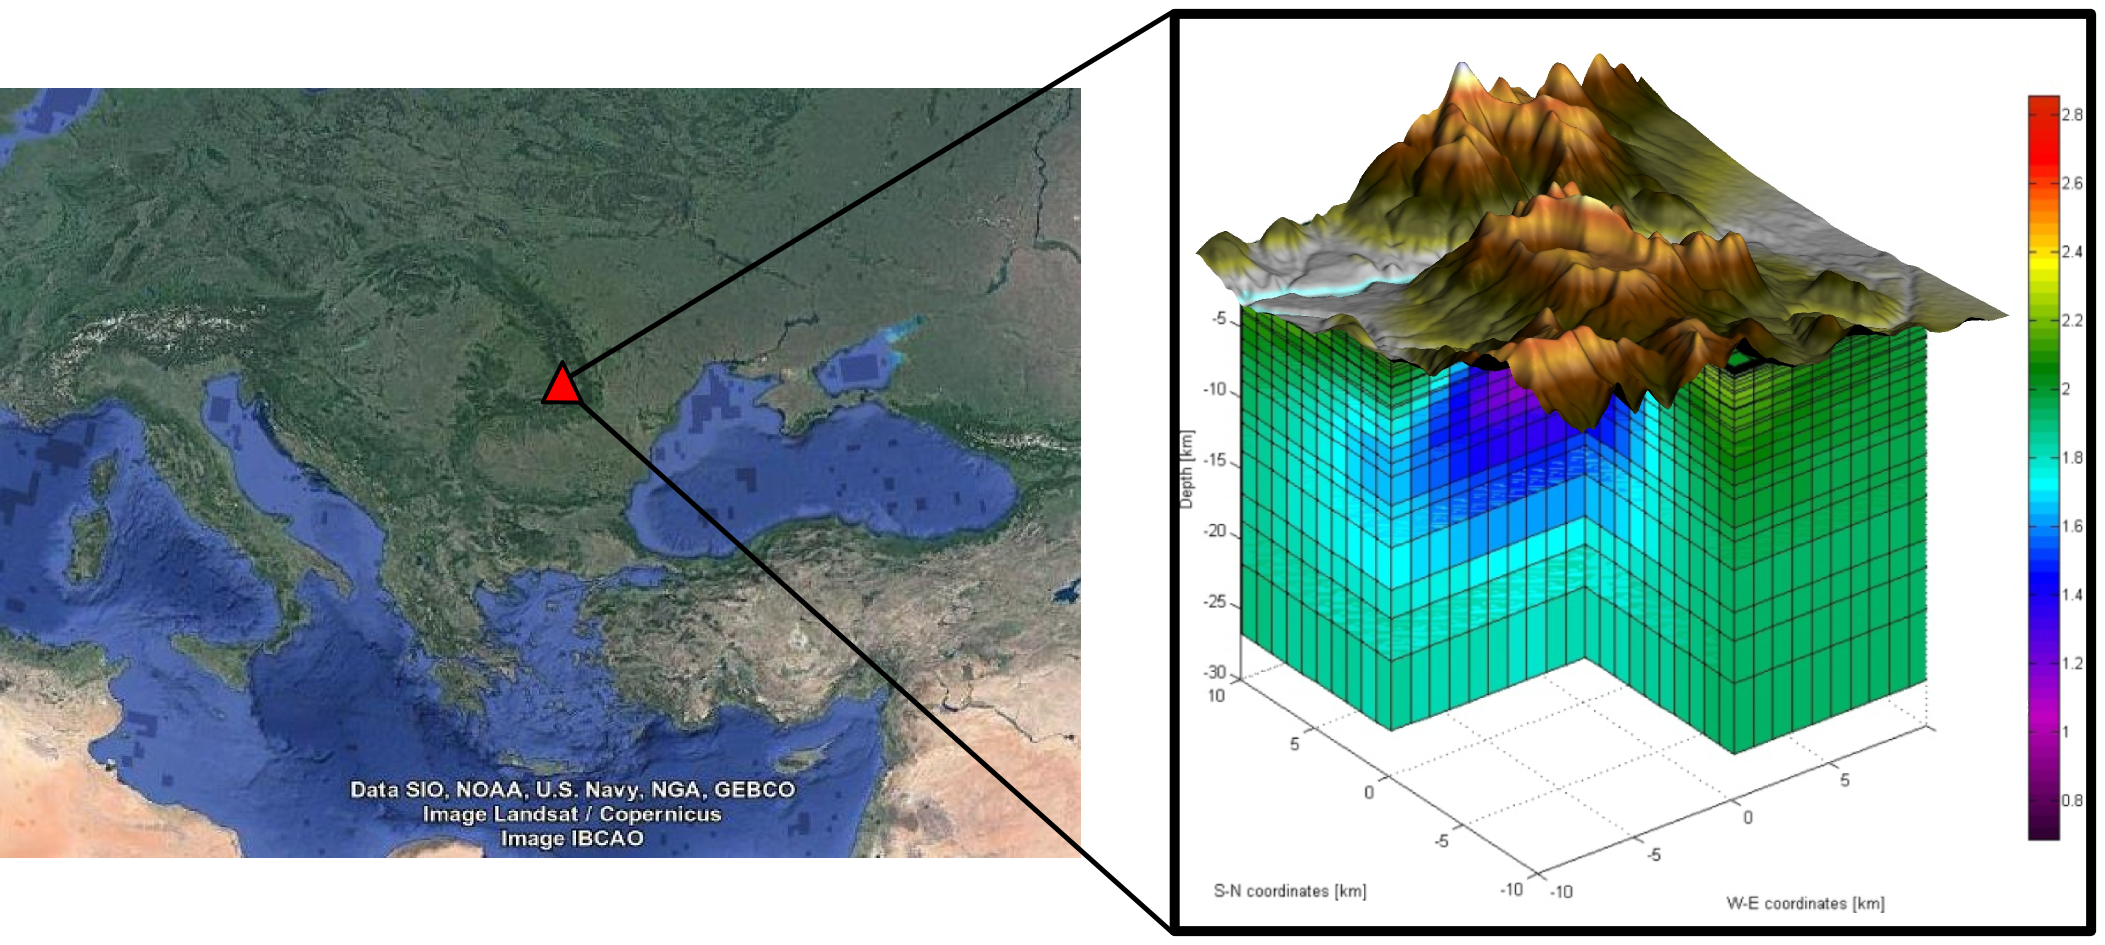
\includegraphics[width=0.45\textwidth]{google_earth_csomad_harangi.png}
    \caption{Location of the Ciomadul volcano and the low-resistivity anomaly under it. The red triangle denotes the volcano. Colorscale shows $\si{\ohm\meter}$ values on logarithmic scale. \cite{Harangi2015}}
\end{figure}

%-----------------------------------------------------------------------
% METHOD
%-----------------------------------------------------------------------

\sectitle{2. Method}

We used the method of Multi-Temporal InSAR (MTInSAR)to estimate east-west and vertical surface deformation velocities in the vicinity of the Coimadul volcano. The simplified version of the processing chain can be seen below:

\begin{enumerate}
    \item Focusing of raw Envisat images into SAR images.
    \item Coregistration of SAR images to a single master image. Creation of interferograms (IFGs), removal of topographic and flat-earth phase.
    \item \stamps \cite{Hooper2008} processing: selection of pixels with ``stable'' phase values (Persistent Scatterers, PSs) based on the probability density functions of temporal coherence values of random and filtered phase; weeding of PSs with high noise std.; unwrapping and calculation of LOS deformation time series and velocities
    \item \daisy processing: calculating the position of dominant points (DPs) in selected clusters of ASC and DSC PS points; LOS velocities of ASC and DSC points are interpolated to the DP positions integration of LOS velocities resulting in the EW and UP velocity components; selection of a reference area; the mean EW and UP velocity components of DPs inside the reference area are calculated and subtracted from all DPs
    \item Analysis and visualisation of integrated velocities.
\end{enumerate}

%-----------------------------------------------------------------------
% Envisat Images
%-----------------------------------------------------------------------

\sectitle{3. Envisat images}

\begin{itemize}
    \item 23 ascending and 32 descending archived raw SAR Envisat images
    \item timespan: 2002-2010; large temporal and spatial baselines $\rightarrow$ SBAS method instead of PS
    \item selection of coherent IFGs, connecting them to the master image with less coherent IFGs $\rightarrow$ SBAS network for ASC and DSC images.
\end{itemize}

\begin{figure}[H]
    \begin{minipage}[t]{0.25\textwidth}
        \centering
        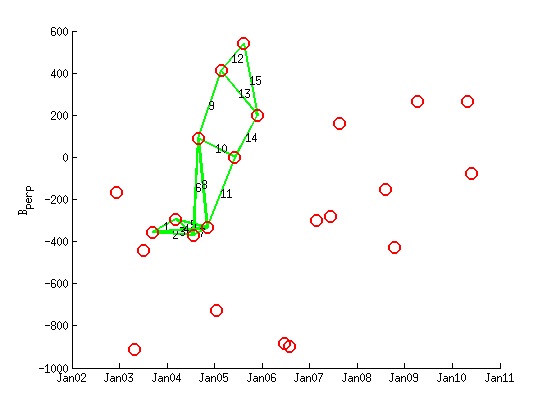
\includegraphics[]{asc_sbas_select.png}
        \caption{SBAS network of ASC IFGs}
    \end{minipage}
    \begin{minipage}[t]{0.25\textwidth}
        \centering
        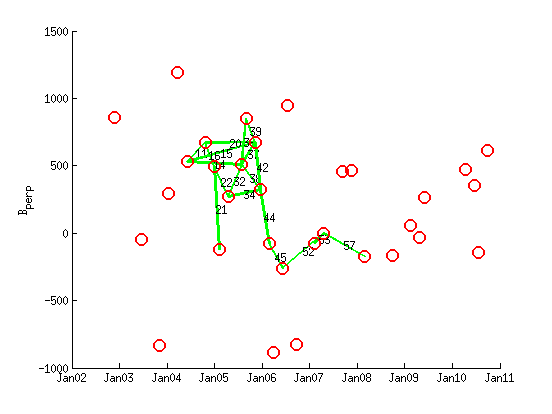
\includegraphics[]{dsc_sbas_select.png}
        \caption{SBAS network of DSC IFGs}
    \end{minipage}
\end{figure}

%-----------------------------------------------------------------------
% RESULTS
%-----------------------------------------------------------------------

\sectitle{4. Results}

Output LOS velocities have been filtered based on their relative standard deviations (``standard deviation of mean velocity'' / ``mean velocity''). Datapoints with rel. std. > 25\% were discarded.

\begin{figure}[H]
    \centering
    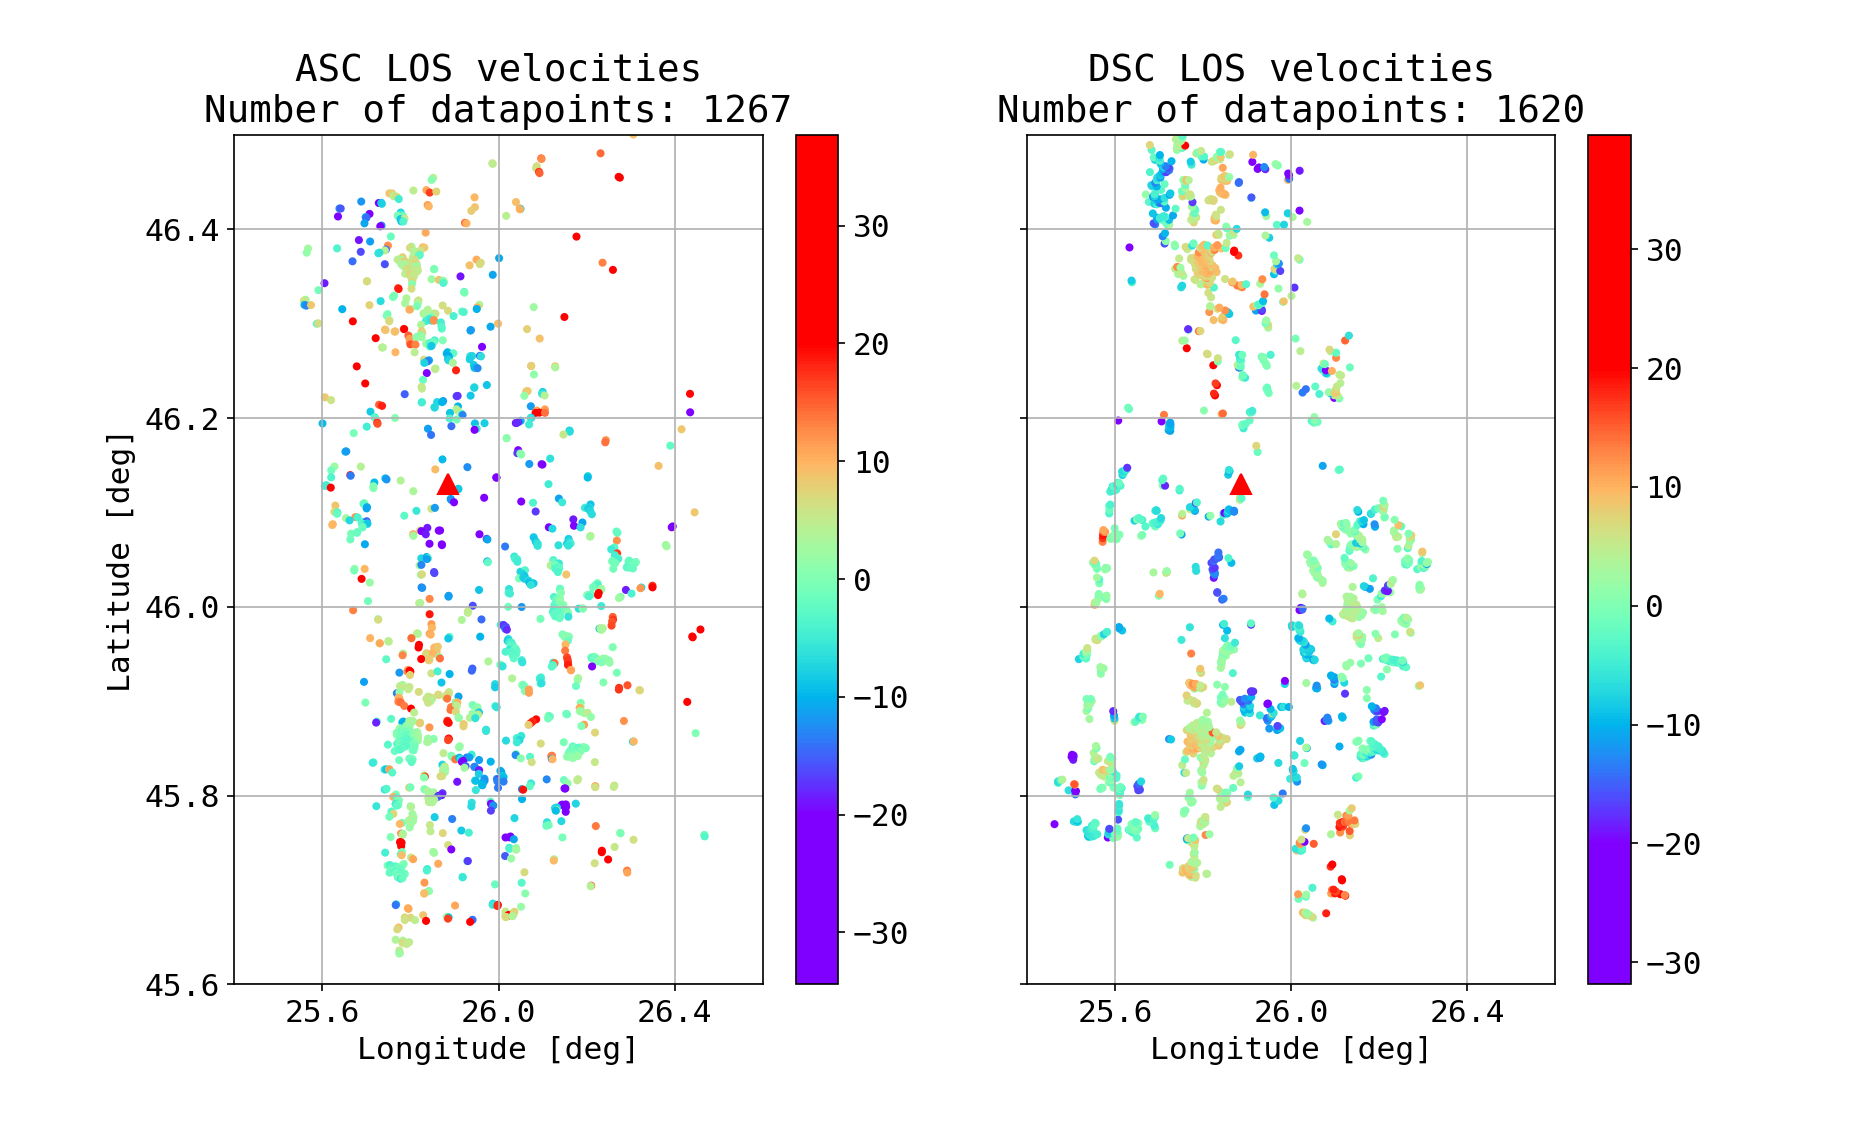
\includegraphics[width=0.4\textwidth]{asc_dsc_los.png}
    \caption{Ascending and Descending LOS velocities. Red triangle shows the position of Ciomadul volcano.}
\end{figure}

\begin{figure}[H]
    \centering
    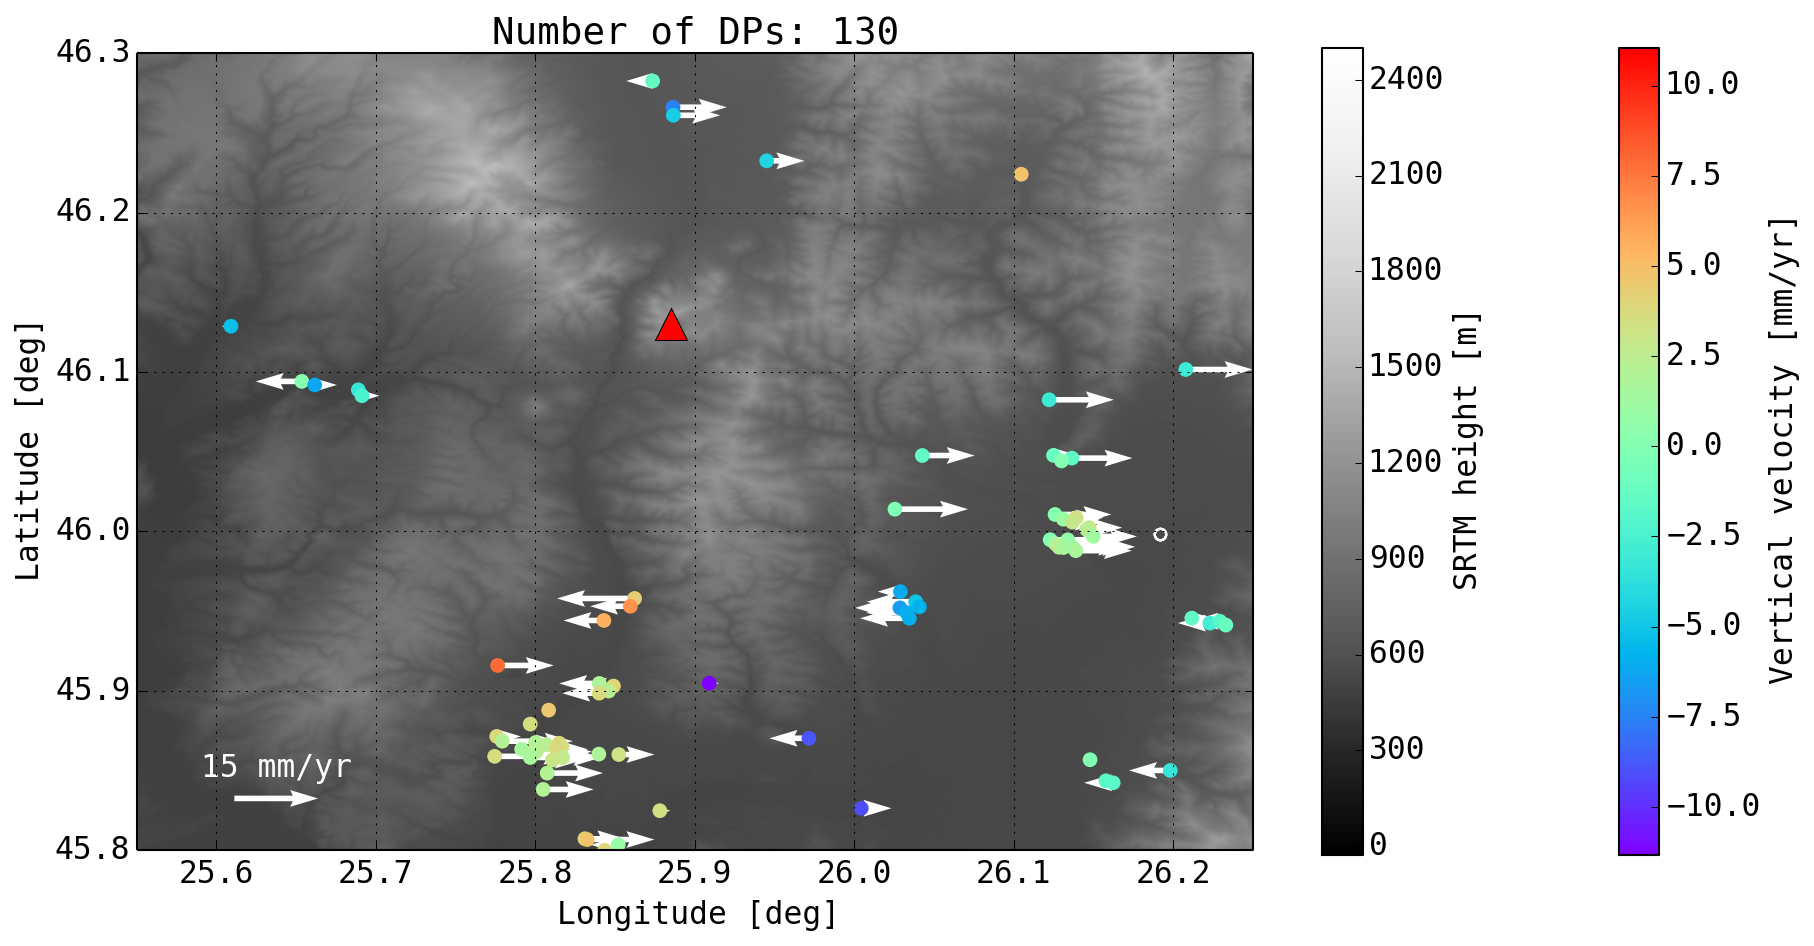
\includegraphics[width=0.4\textwidth]{dp.png}
    \caption{Integrated East-West and vertical velocities with the SRTM DEM in the background. Red triangle shows the position of Ciomadul volcano, green empty circles denote the positions of the reference points.}
\end{figure}

\begin{itemize}
    \item inhomogeneous PS distribution, \stamps discarded many pixels because of the incoherent areas in many IFGs
    \item some outlier datapoints are present in ASC and DSC PS points
    \item IFGs with large temporal and spatial baselines, heavily vegetated area $\rightarrow$ multi-temporal InSAR struggles to find reliable PS points
    \item the velocity field more or less corresponds to the usual geological interpretation of the Carpathian Bend Zone; i.e. eastward movement originating from Adriatic Plate push, subsidence of basins due to compaction
\end{itemize}

%-----------------------------------------------------------------------
% CONCLUSIONS & PRACTICAL ADVICES
%-----------------------------------------------------------------------

\sectitle{5. Conclusions and Practical advices}

Deriving surface deformation velocities with MTInSAR in a vegetated area using IFGs with large temporal and spatial baselines is major challange. Due to the incoherence in IFGs, PS point densitiy is low and unwrapping errors contaminate LOS deformation velocities thus results should be interpreted with care. The recently launched Sentinel-1A/B mission provides small temporal and spatial baselines, however a long time series is required for the analysis of small magnitude surface deformation velocities.

\vspace{25pt}
Below are some useful advices for processing incoherent IFGs with \stamps:
\begin{enumerate}
    \item Use SBAS method to minimize temporal and spatial baselines. Select coherent IFGs and try to create an SBAS network using less coherent IFGs.
    \item Carry out the \stamps processing using the default processing parameters. The most important parameter you may want to play with is the number of PS pixels included in the unwrapping. Try to weed out noisy pixels and use larger resampling grid sizes (e.g. $\num{300}-\SI{400}{\meter}$). Be careful, if you throw away too many PSs, \stamps might not be able to correctly unwrap the phase values.
    \item Use the ``3D'' unwrapping method instead of ``3D-quick''.
    \item At the end of the processing \stamps outputs the LOS deformation velocity values, their standard deviations can be calculated as well. Filter out PSs, that have large relative standard deviation values or use your preferred data weeding method.
\end{enumerate}
\vspace{30pt}
{\color{blue} \large \daisy source code can be downloaded at: \url{http://ggki.hu/~banyai/}}

\normalfont
\bibliographystyle{plain}
\bibliography{/home/istvan/work/insar/insar}

\end{multicols}

\end{document}
